\documentclass[border=6pt]{standalone}
\usepackage{fontspec,unicode-math}
\setmainfont{Noto Serif}
\setmathfont{STIXTwoMath-Regular.otf}
\usepackage{tikz}
\usetikzlibrary{arrows.meta,calc,patterns,decorations.markings,decorations.pathmorphing,decorations.pathreplacing}
\tikzset{lev/.style={line width=1.2pt,line cap=butt},
 fine/.style={line width=.54pt},light/.style={line width=.37pt},
 curve/.style={line width=1.2pt,line cap=round,line join=round},
 ax/.style={line width=.62pt,-{Latex[length=2.1mm,width=1.15mm]}},
 ray/.style={line width=.58pt,-{Latex[length=1.85mm,width=.95mm]},shorten >=1.4pt,shorten <=1.4pt},
 dim/.style={line width=.52pt,{Latex[length=1.6mm,width=.85mm]}-{Latex[length=1.6mm,width=.85mm]}},
 flow/.style={line width=.60pt,postaction={decorate},decoration={markings,mark=at position .62 with {\arrow{Latex[length=1.8mm,width=.95mm]}}}},
 lab/.style={font=\fontsize{12}{14.4}\selectfont,inner sep=1.6pt},
 small/.style={font=\fontsize{10.5}{12.5}\selectfont,inner sep=1.3pt},
 tinylabel/.style={font=\fontsize{9.2}{11}\selectfont,inner sep=1.0pt},
 panel/.style={font=\fontsize{12}{14.4}\selectfont\itshape,inner sep=1.5pt}}
\pagestyle{empty}
\begin{document}
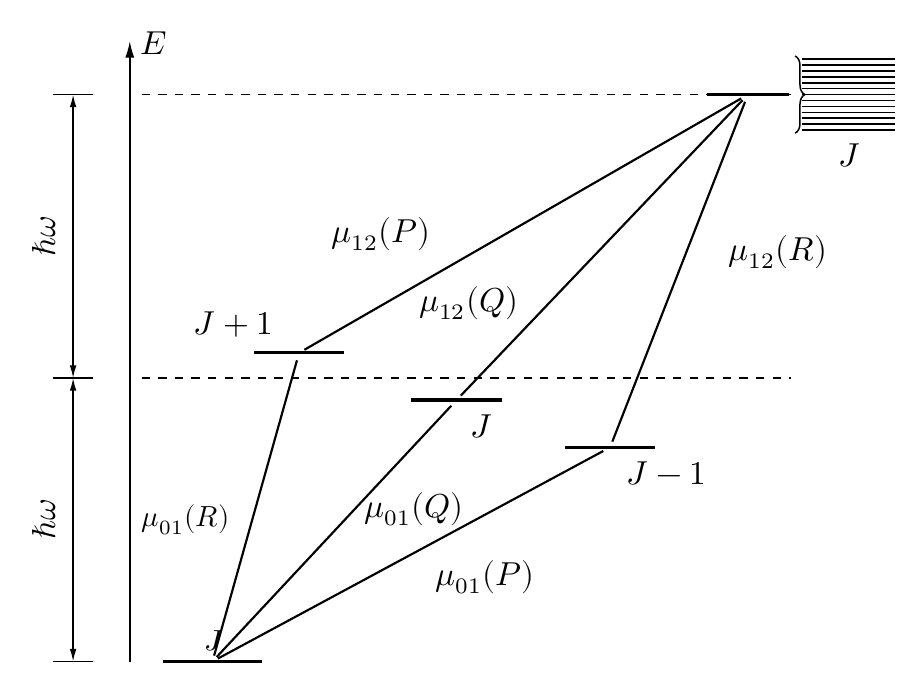
\begin{tikzpicture}[x=1cm,y=1cm,line join=round]
\draw[ax] (0.30000,0.35000)--(0.30000,8.23000);
\node[lab,anchor=west] at (0.37000,8.20000) {$E$};
\draw[fine,dashed] (0.45000,3.95000)--(8.70000,3.95000);
\draw[fine,dashed] (0.45000,7.55000)--(8.70000,7.55000);
\coordinate (initial) at (1.35000,0.35000);
\draw[lev] (0.72500,0.35000)--(1.97500,0.35000);
\node[small,anchor=south] at (1.35000,0.43000) {$J$};
\coordinate (interR) at (2.45000,4.27000);
\draw[lev] (1.87500,4.27000)--(3.02500,4.27000);
\node[lab,anchor=south east] at (2.18000,4.41000) {$J+1$};
\coordinate (interQ) at (4.45000,3.67000);
\draw[lev] (3.87500,3.67000)--(5.02500,3.67000);
\node[lab,anchor=north west] at (4.57000,3.55000) {$J$};
\coordinate (interP) at (6.40000,3.07000);
\draw[lev] (5.82500,3.07000)--(6.97500,3.07000);
\node[lab,anchor=north west] at (6.55000,2.95000) {$J-1$};
\coordinate (final) at (8.15000,7.55000);
\draw[lev] (7.62500,7.55000)--(8.67500,7.55000);
\draw[fine] (8.84000,7.10000)--(10.02000,7.10000);
\draw[fine] (8.84000,7.17500)--(10.02000,7.17500);
\draw[fine] (8.84000,7.25000)--(10.02000,7.25000);
\draw[fine] (8.84000,7.32500)--(10.02000,7.32500);
\draw[fine] (8.84000,7.40000)--(10.02000,7.40000);
\draw[fine] (8.84000,7.47500)--(10.02000,7.47500);
\draw[fine] (8.84000,7.55000)--(10.02000,7.55000);
\draw[fine] (8.84000,7.62500)--(10.02000,7.62500);
\draw[fine] (8.84000,7.70000)--(10.02000,7.70000);
\draw[fine] (8.84000,7.77500)--(10.02000,7.77500);
\draw[fine] (8.84000,7.85000)--(10.02000,7.85000);
\draw[fine] (8.84000,7.92500)--(10.02000,7.92500);
\draw[fine] (8.84000,8.00000)--(10.02000,8.00000);
\draw[fine,decorate,decoration={brace,amplitude=3.5pt,mirror}] (8.75,7.06)--(8.75,8.04);
\node[lab,anchor=north] at (9.42000,6.99000) {$J$};
\draw[fine,line width=.78pt,shorten <=2.2pt,shorten >=2.8pt] (initial)--(interR);
\draw[fine,line width=.78pt,shorten <=2.2pt,shorten >=2.8pt] (interR)--(final);
\draw[fine,line width=.78pt,shorten <=2.2pt,shorten >=2.8pt] (initial)--(interQ);
\draw[fine,line width=.78pt,shorten <=2.2pt,shorten >=2.8pt] (interQ)--(final);
\draw[fine,line width=.78pt,shorten <=2.2pt,shorten >=2.8pt] (initial)--(interP);
\draw[fine,line width=.78pt,shorten <=2.2pt,shorten >=2.8pt] (interP)--(final);
\node[small,anchor=east] at (1.62000,2.15000) {$\mu_{01}(R)$};
\node[lab,anchor=west] at (3.22000,2.28000) {$\mu_{01}(Q)$};
\node[lab,anchor=west,fill=white] at (4.12000,1.42000) {$\mu_{01}(P)$};
\node[lab,anchor=east,fill=white] at (4.18000,5.78000) {$\mu_{12}(P)$};
\node[lab,anchor=east] at (5.30000,4.90000) {$\mu_{12}(Q)$};
\node[lab,anchor=west] at (7.84000,5.55000) {$\mu_{12}(R)$};
\draw[dim] (-0.42000,0.35000)--(-0.42000,3.95000);
\draw[fine] (-0.68000,0.35000)--(-0.17000,0.35000);
\draw[fine] (-0.68000,3.95000)--(-0.17000,3.95000);
\node[lab,anchor=south,rotate=90] at (-0.58000,2.15000) {$\hbar\omega$};
\draw[dim] (-0.42000,3.95000)--(-0.42000,7.55000);
\draw[fine] (-0.68000,3.95000)--(-0.17000,3.95000);
\draw[fine] (-0.68000,7.55000)--(-0.17000,7.55000);
\node[lab,anchor=south,rotate=90] at (-0.58000,5.75000) {$\hbar\omega$};
\end{tikzpicture}
\end{document}
